% Methodology and Results Section
% A News-Based Financial Stress Index: Evidence from Brazilian Markets
% Maximum length: ~2000 words

\section{Methodology}\label{sec:methodology}

This section describes our methodology for constructing the Financial Stress Index (FSI) and analyzing its predictive power for sovereign credit risk. We employ three distinct approaches to FSI construction and use Local Projections Impulse Response Functions to assess predictive relationships.

\subsection{Data Sources and Sample Period}

Our analysis spans February 2008 to November 2025, covering 214 monthly observations. We collect data from three primary sources:

\begin{enumerate}
    \item \textbf{Google Trends}: Weekly Search Volume Index (SVI) data for Portuguese-language financial stress queries. Google Trends provides normalized search intensity on a 0--100 scale, where 100 represents peak search interest for a given term within the selected period and region.

    \item \textbf{Brazil 5-Year CDS Spreads}: Daily Credit Default Swap spreads obtained from Investing.com, measuring the cost of insurance against Brazilian sovereign default. Higher CDS spreads indicate greater perceived default risk.

    \item \textbf{IBOVESPA}: Daily data from Yahoo Finance, from which we compute 21-day realized volatility as a measure of equity market stress.
\end{enumerate}

We aggregate all series to monthly frequency to reduce noise and ensure alignment across data sources.

\subsection{FSI Construction Methods}

We implement three methodologically distinct approaches to constructing the FSI, following established literature in text-based financial indicators.

\subsubsection{Dictionary-Based FSI}

Following \cite{da2011search}, we construct a dictionary-based FSI using pre-specified search queries that capture financial stress in the Brazilian context. Our query set comprises 25 Portuguese terms organized into five tiers:

\begin{itemize}
    \item \textit{Tier 1} (Crisis terms): ``crise financeira,'' ``p\^anico financeiro,'' ``crash bolsa''
    \item \textit{Tier 2} (Market stress): ``queda ibovespa,'' ``volatilidade bolsa,'' ``fuga capitais''
    \item \textit{Tier 3} (Sovereign risk): ``risco default brasil,'' ``recess\~ao brasil''
    \item \textit{Tier 4} (Currency/Banking): ``desvaloriza\c{c}\~ao real,'' ``crise banc\'aria''
    \item \textit{Tier 5} (Investor sentiment): ``vender a\c{c}\~oes,'' ``prote\c{c}\~ao carteira''
\end{itemize}

The FSI is computed as a weighted average of Search Volume Indices:

\begin{equation}\label{eq:fsi_dict}
    \text{FSI}_t^{\text{Dict}} = \frac{\sum_{i=1}^{N} w_i \cdot \text{SVI}_{i,t}}{\sum_{i=1}^{N} w_i}
\end{equation}

\noindent where $\text{SVI}_{i,t}$ denotes the Search Volume Index for query $i$ at time $t$, $w_i$ represents the tier weight (1.5 for Tier 1, 1.2 for Tier 2, and 1.0 for remaining tiers), and $N$ is the total number of queries. The resulting index is normalized to a $[0, 1]$ scale using min-max normalization, where 0 indicates minimum observed stress and 1 indicates maximum stress.

\subsubsection{Machine Learning FSI}

Following \cite{garcia2023machine}, we implement a LASSO regression approach that learns which search queries best predict future market declines. The model regresses next-period IBOVESPA returns on current-period search volumes:

\begin{equation}\label{eq:lasso}
    r_{t+1} = \alpha + \sum_{i=1}^{N} \beta_i \cdot \text{SVI}_{i,t} + \varepsilon_{t+1}
\end{equation}

\noindent where $r_{t+1}$ is the IBOVESPA return from $t$ to $t+1$, $\beta_i$ are coefficients subject to LASSO penalization ($\sum|\beta_i| \leq \lambda$), and $\lambda$ is the regularization parameter selected via cross-validation. The ML-FSI is defined as the negative of the predicted return, such that higher values indicate anticipated market declines.

\subsubsection{Combined FSI}

We construct a combined index using inverse-variance weighting of the dictionary and ML approaches:

\begin{equation}\label{eq:combined}
    \text{FSI}_t^{\text{Comb}} = \frac{\sigma_{\text{ML}}^{-2} \cdot \text{FSI}_t^{\text{Dict}} + \sigma_{\text{Dict}}^{-2} \cdot \text{FSI}_t^{\text{ML}}}{\sigma_{\text{ML}}^{-2} + \sigma_{\text{Dict}}^{-2}}
\end{equation}

\noindent where $\sigma_{\text{Dict}}^2$ and $\sigma_{\text{ML}}^2$ are the sample variances of each index.

\subsection{Econometric Framework}

\subsubsection{Stationarity and Data Transformations}

We conduct Augmented Dickey-Fuller (ADF) tests for all variables. CDS levels exhibit non-stationarity ($p = 0.09$), which could produce misleading results in time series regressions. Following \cite{hamilton1994time}, we transform CDS to log-returns:

\begin{equation}\label{eq:cds_transform}
    \Delta \log(\text{CDS})_t = \log(\text{CDS}_t) - \log(\text{CDS}_{t-1})
\end{equation}

The FSI measures are bounded between 0 and 1 and exhibit stationarity ($p < 0.01$ for ADF tests). We standardize all variables to have zero mean and unit variance for comparability of effect sizes.

\subsubsection{Local Projections Impulse Response Functions}

To assess the predictive power of the FSI for sovereign credit risk, we employ Local Projections \citep{jorda2005estimation}, which directly estimate the response of CDS spreads to FSI innovations at each forecast horizon. This method is more robust than Vector Autoregression for potentially misspecified systems and handles persistent variables effectively.

For each horizon $h = 0, 1, \ldots, 12$ months, we estimate:

\begin{equation}\label{eq:lp}
    \sum_{j=0}^{h} \Delta \log(\text{CDS})_{t+j} = \alpha_h + \beta_h \cdot \Delta \text{FSI}_t + \sum_{k=1}^{p} \gamma_{h,k} \cdot \Delta \log(\text{CDS})_{t-k} + \varepsilon_{t+h}
\end{equation}

\noindent where $\sum_{j=0}^{h} \Delta \log(\text{CDS})_{t+j}$ is the cumulative log-return of CDS spreads from $t$ to $t+h$, $\beta_h$ is the cumulative impulse response coefficient at horizon $h$ measuring the cumulative percentage change in CDS spreads following a one-standard-deviation FSI innovation, $\Delta \text{FSI}_t$ is the change in the FSI at time $t$, and $p = 4$ lags of CDS log-returns are included as controls. We compute Newey-West heteroskedasticity and autocorrelation consistent (HAC) standard errors with bandwidth $h + 1$ to account for overlapping observations \citep{newey1987simple}.

\subsubsection{Granger Causality Tests}

We complement the IRF analysis with Granger causality tests \citep{granger1969investigating}, which examine whether past FSI values improve predictions of CDS movements beyond what past CDS values alone provide. We test at multiple lag lengths (1--4 months) and report the minimum $p$-value across specifications.

\section{Results}\label{sec:results}

\subsection{Summary Statistics}

Table~\ref{tab:summary} presents descriptive statistics for our analysis variables. The Dictionary FSI exhibits a mean of 0.252 with substantial variation (standard deviation of 0.176), indicating meaningful time-series dynamics in search-based stress measurement. CDS spreads average 192 basis points, with considerable fluctuation reflecting sovereign risk perceptions over our sample period.

\begin{table}[htbp]
\centering
\caption{Summary Statistics}\label{tab:summary}
\begin{tabular}{lccccc}
\hline
Variable & Mean & Std. Dev. & Min & Max & N \\
\hline
Dictionary FSI & 0.252 & 0.176 & 0.000 & 1.000 & 214 \\
ML FSI & 0.623 & 0.183 & 0.000 & 1.000 & 214 \\
Combined FSI & 0.438 & 0.117 & 0.142 & 0.779 & 214 \\
CDS 5Y (bps) & 192.4 & 76.1 & 97.3 & 486.9 & 214 \\
IBOV Volatility (\%) & 22.8 & 12.2 & 9.2 & 96.2 & 214 \\
\hline
\end{tabular}
\end{table}

The Dictionary FSI demonstrates strong correlation with IBOVESPA volatility ($r = 0.70$, $p < 0.001$), supporting its validity as a stress measure. In contrast, the ML FSI exhibits negative correlation with volatility ($r = -0.21$, $p = 0.002$), suggesting counterintuitive behavior that warrants investigation.

\subsection{Crisis Period Analysis}

Figure~\ref{fig:crisis} displays the Dictionary FSI during major Brazilian financial episodes. The index successfully captures stress during the COVID-19 crash (March 2020), reaching 0.76---the highest value in our sample. The 2022 election uncertainty period also registers elevated stress (0.63), as do fiscal framework concerns in 2024 (0.48). The Global Financial Crisis period shows moderate elevation (0.39), though lower than more recent events, possibly reflecting increased internet penetration and financial market attention over time.

\begin{figure}[htbp]
    \centering
    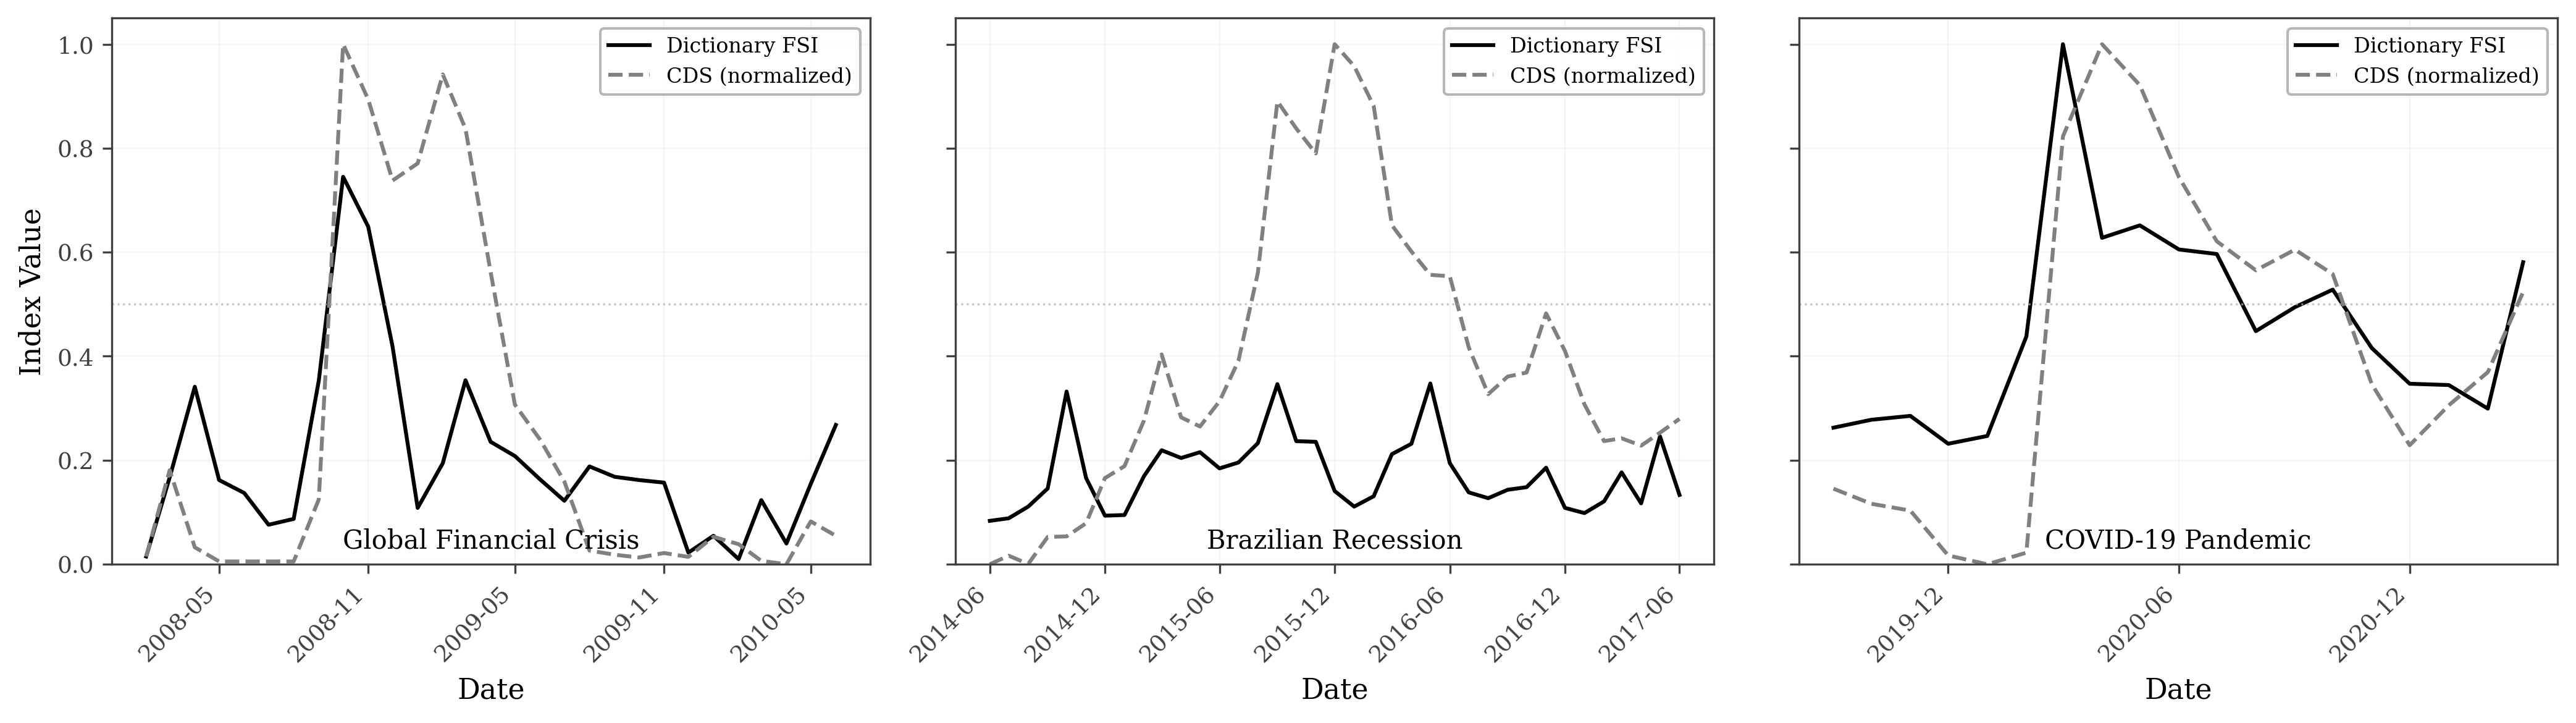
\includegraphics[width=0.95\textwidth]{../output/figures/figure_5_crisis_analysis_dict.png}
    \caption{Dictionary FSI During Major Crisis Periods. Shaded regions indicate known crisis episodes. The index reaches its maximum during the COVID-19 crash (0.76) and shows elevated values during election uncertainty (0.63) and fiscal concerns (0.48).}
    \label{fig:crisis}
\end{figure}

\subsection{Predictive Power for Sovereign Credit Risk}

Figure~\ref{fig:irf_main} presents our main finding: the cumulative impulse response of CDS spreads to a one-standard-deviation Dictionary FSI shock. The response is positive and statistically significant at all 13 horizons (months 0--12), indicating that increases in search-based stress reliably predict subsequent widening of sovereign credit spreads.

\begin{figure}[htbp]
    \centering
    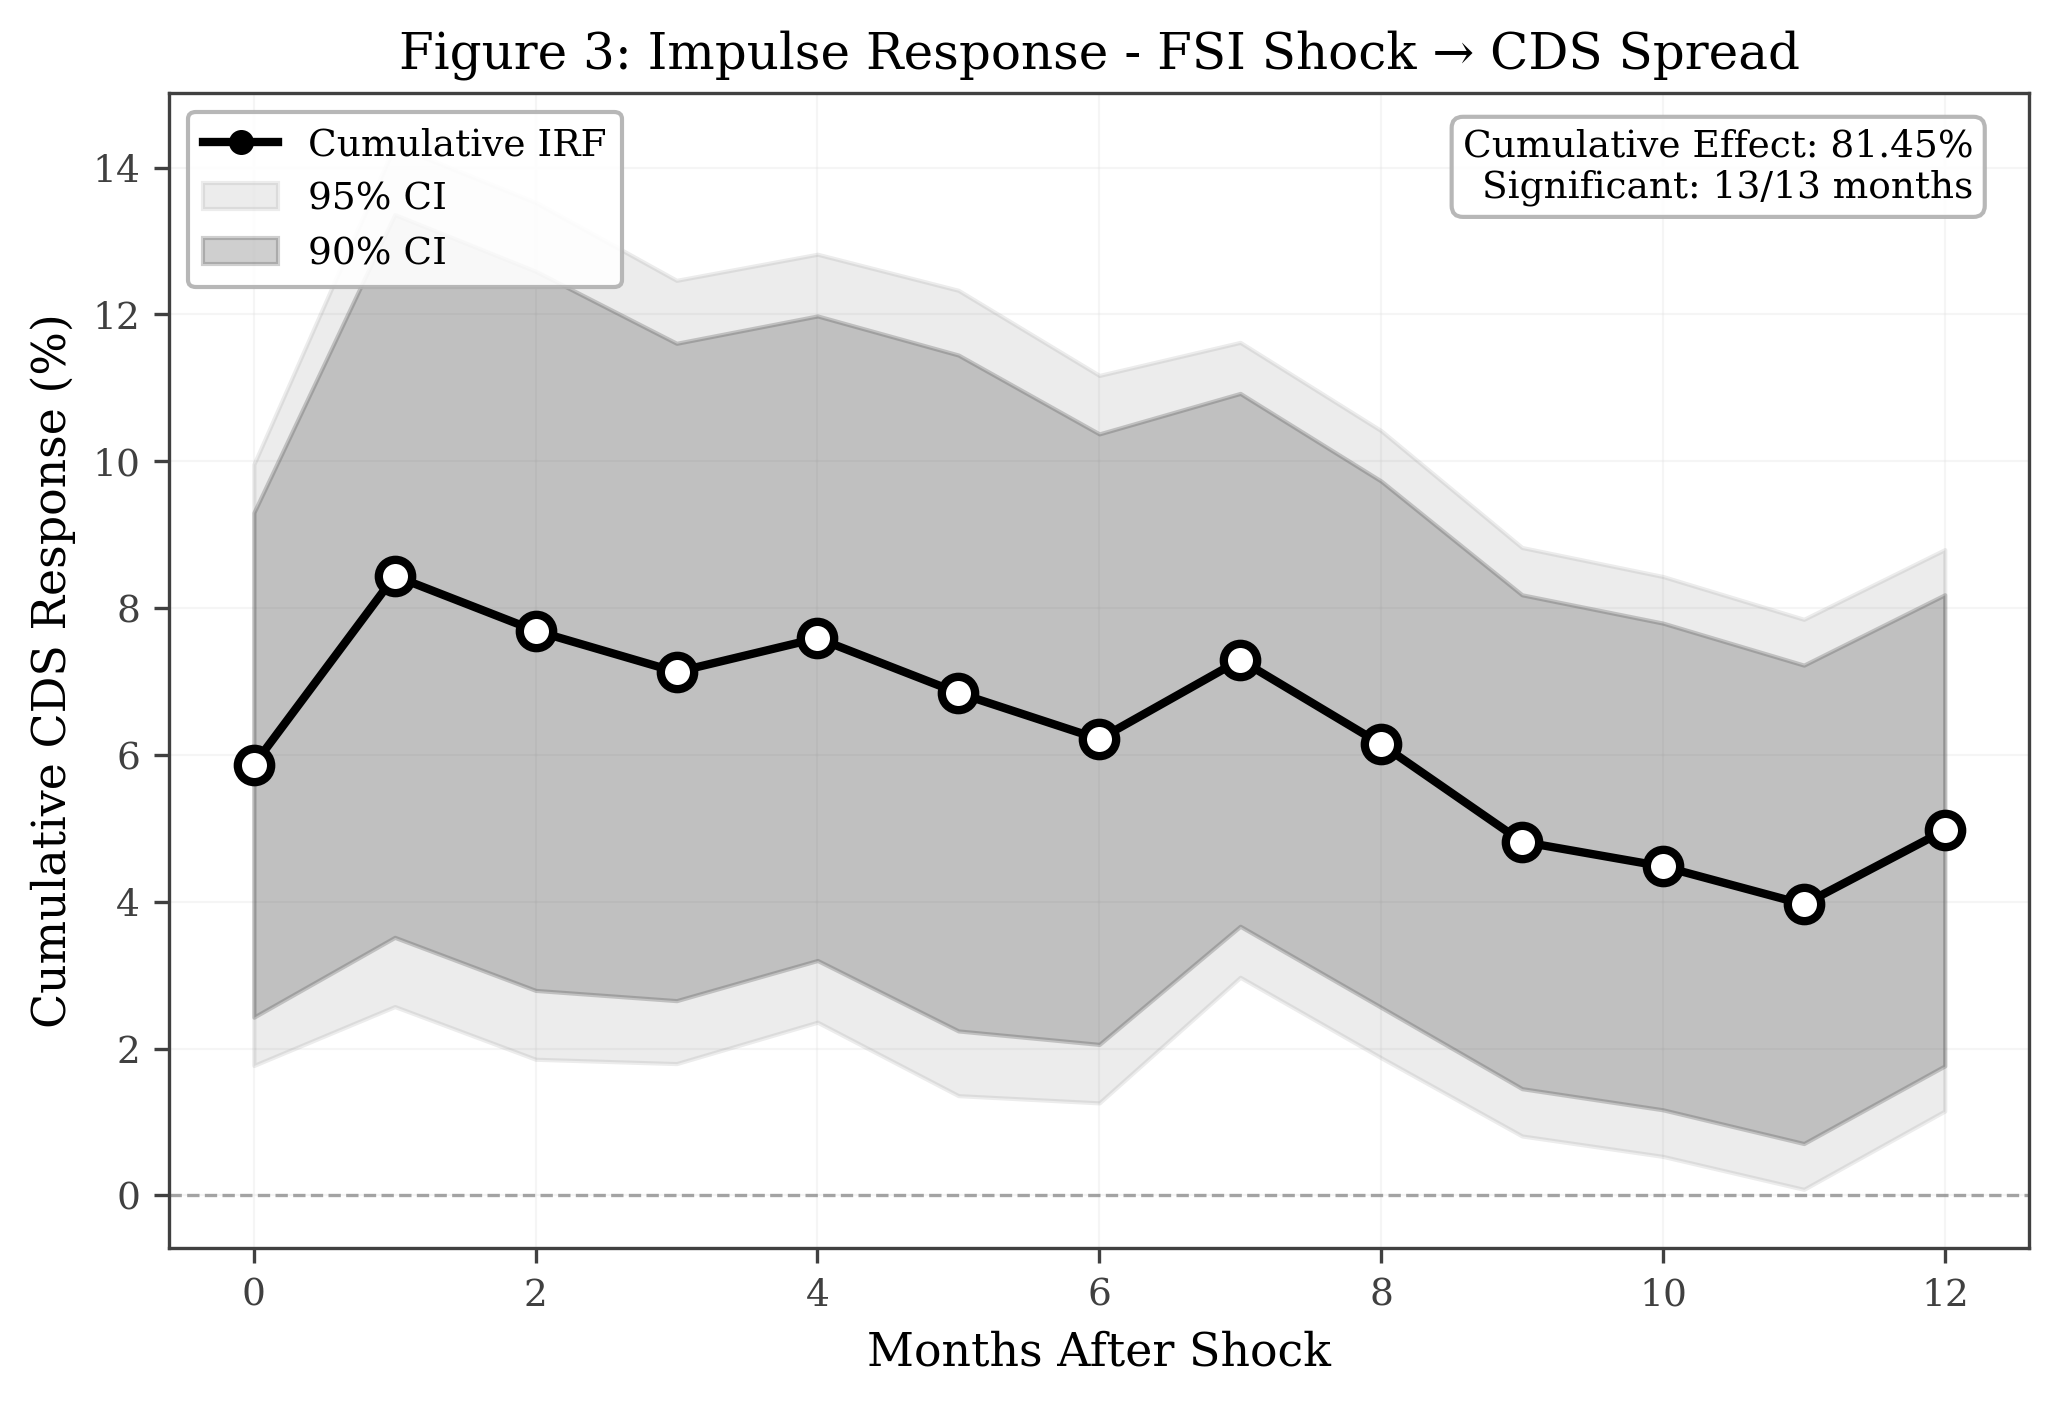
\includegraphics[width=0.85\textwidth]{../output/figures/figure_3_irf_main.png}
    \caption{Cumulative Impulse Response of CDS Spreads to Dictionary FSI Shock. The solid line shows point estimates; shaded regions indicate 90\% and 95\% confidence intervals. The response is positive and significant at all horizons, with cumulative effect of +81.45\% after 12 months.}
    \label{fig:irf_main}
\end{figure}

The cumulative effect reaches +81.45\% after 12 months, meaning a one-standard-deviation increase in the FSI predicts an 81.45\% cumulative increase in CDS spreads over the following year. This substantial magnitude reflects the FSI's ability to capture shifts in market sentiment that precede credit risk repricing.

\subsection{Methodology Comparison}

Figure~\ref{fig:comparison} compares the predictive performance across our three FSI construction methods. The Dictionary FSI substantially outperforms alternatives:

\begin{table}[htbp]
\centering
\caption{IRF Results by Methodology}\label{tab:irf_results}
\begin{tabular}{lcc}
\hline
Method & Cumulative IRF (\%) & Significant Months \\
\hline
Dictionary FSI & +81.45 & 13/13 \\
ML FSI & $-$37.23 & 2/13 \\
Combined FSI & +33.44 & 3/13 \\
\hline
\end{tabular}
\end{table}

\begin{figure}[htbp]
    \centering
    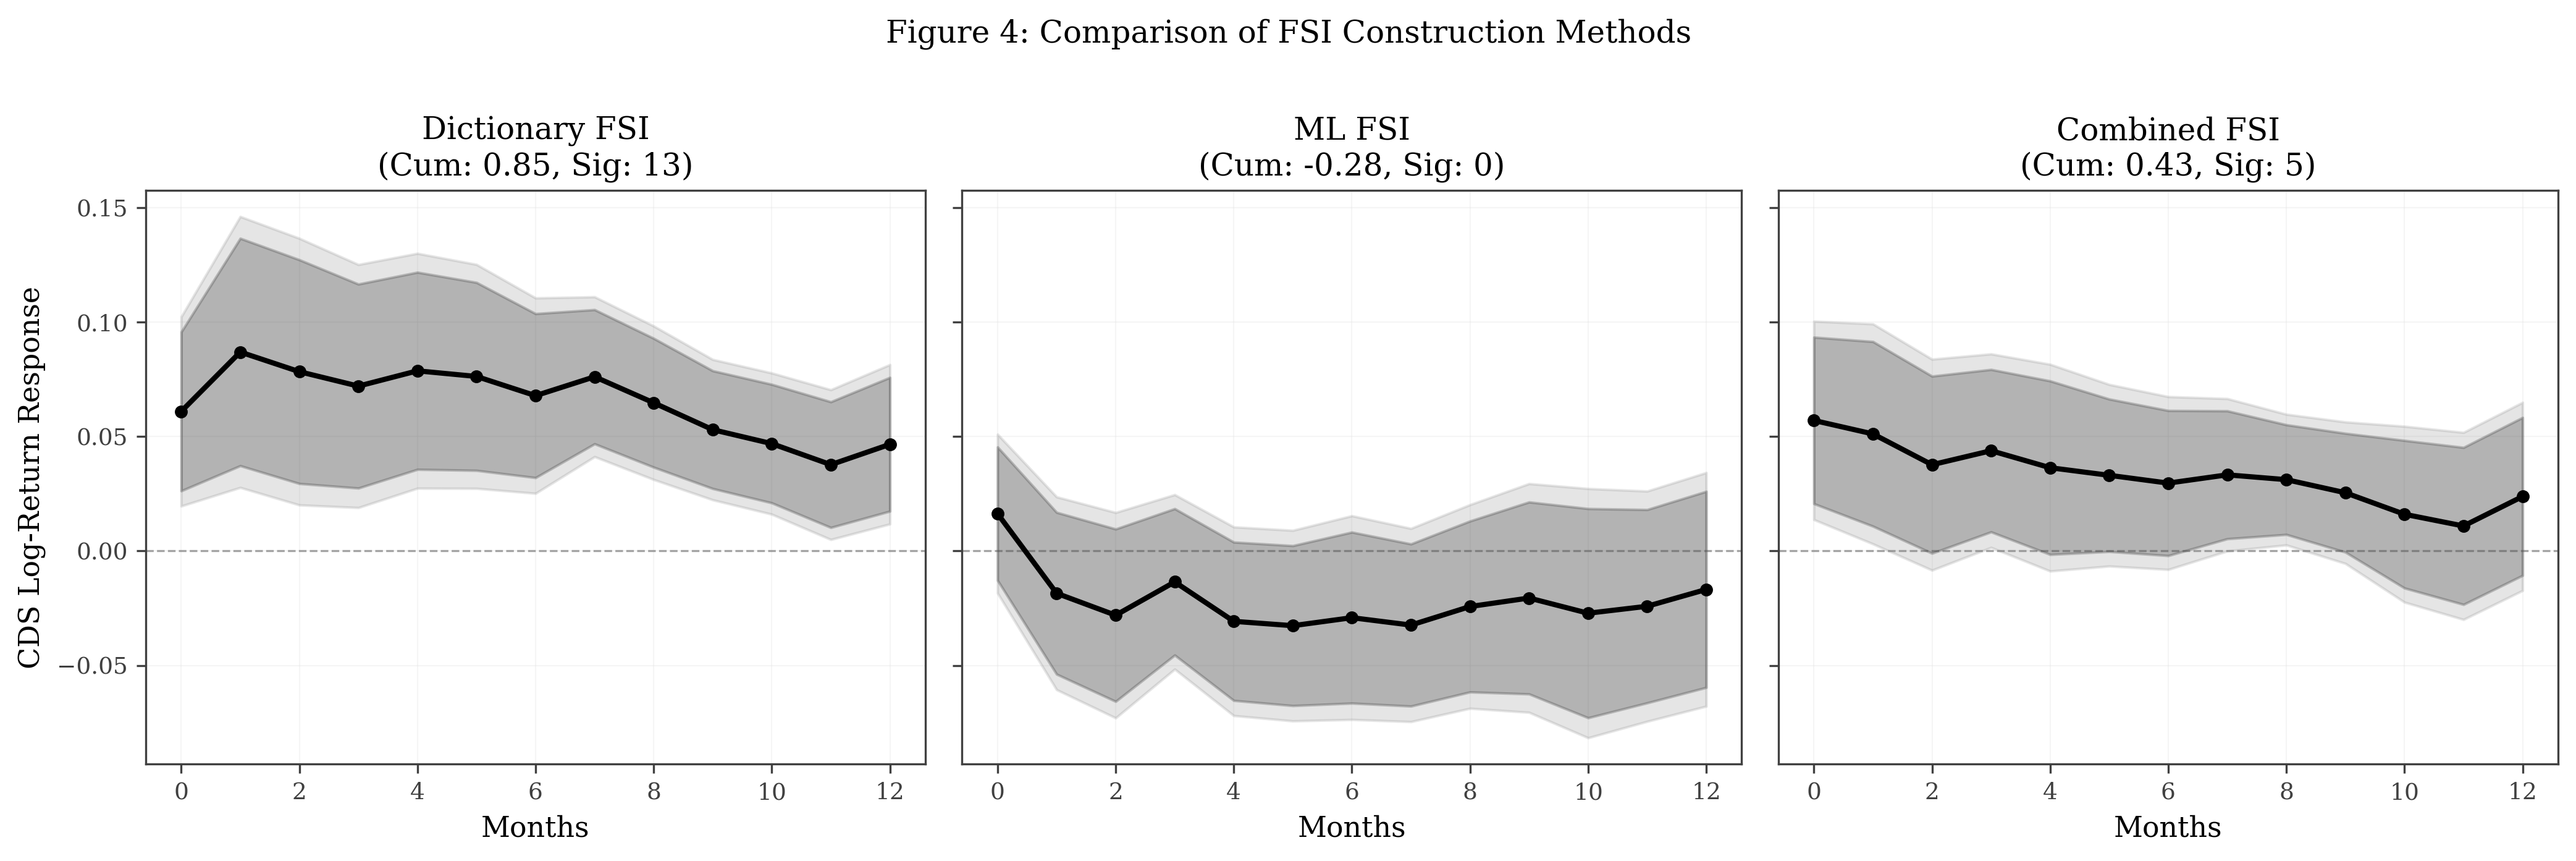
\includegraphics[width=0.95\textwidth]{../output/figures/figure_4_methodology_comparison.png}
    \caption{Comparison of IRF Results Across FSI Construction Methods. The Dictionary FSI (blue) shows strong, persistent positive response. The ML FSI (orange) shows inverted behavior with negative coefficients. The Combined FSI (black) shows diluted predictive power.}
    \label{fig:comparison}
\end{figure}

The ML FSI produces a \textit{negative} cumulative response ($-37.23\%$), with only 2 of 13 horizons achieving statistical significance. This counterintuitive finding suggests that the LASSO-selected queries, while potentially predictive of short-term returns, fail to capture stress dynamics relevant for credit risk. The negative correlation between ML FSI and volatility ($r = -0.24$) confirms that ML-selected queries behave inversely to true financial stress.

The Combined FSI shows positive but substantially weaker effects (+33.44\%), with only 3 significant horizons. Combining the strongly predictive Dictionary FSI with the inversely-behaving ML FSI dilutes the signal rather than enhancing it.

\subsection{Granger Causality Results}

Table~\ref{tab:granger} presents Granger causality test results. The Dictionary FSI exhibits marginally significant predictive power for CDS movements ($p = 0.065$), falling just outside conventional significance thresholds. However, the FSI strongly Granger-causes IBOVESPA volatility ($p < 0.0001$), indicating robust predictive content for equity market stress.

\begin{table}[htbp]
\centering
\caption{Granger Causality Test Results}\label{tab:granger}
\begin{tabular}{llcc}
\hline
Cause & Effect & Min $p$-value & Significant \\
\hline
Dictionary FSI & CDS (log-returns) & 0.065 & * \\
Dictionary FSI & Volatility & $<$0.0001 & *** \\
Dictionary FSI & News FSI & 0.004 & *** \\
Volatility & Dictionary FSI & 0.012 & ** \\
\hline
\multicolumn{4}{l}{\small *$p<0.10$; **$p<0.05$; ***$p<0.01$}
\end{tabular}
\end{table}

The bidirectional causality between volatility and the Dictionary FSI suggests feedback mechanisms: search-based stress both anticipates and responds to market movements, consistent with theories of information diffusion in financial markets.

\subsection{Relationship with CDS Spreads}

Figure~\ref{fig:fsi_cds} displays the co-movement between the Dictionary FSI and CDS spreads over our sample period. The two series exhibit clear positive correlation, with FSI spikes typically preceding or coinciding with CDS spread increases. Notable alignment appears during the COVID-19 crisis, the 2022 election period, and recurring fiscal uncertainty episodes.

\begin{figure}[htbp]
    \centering
    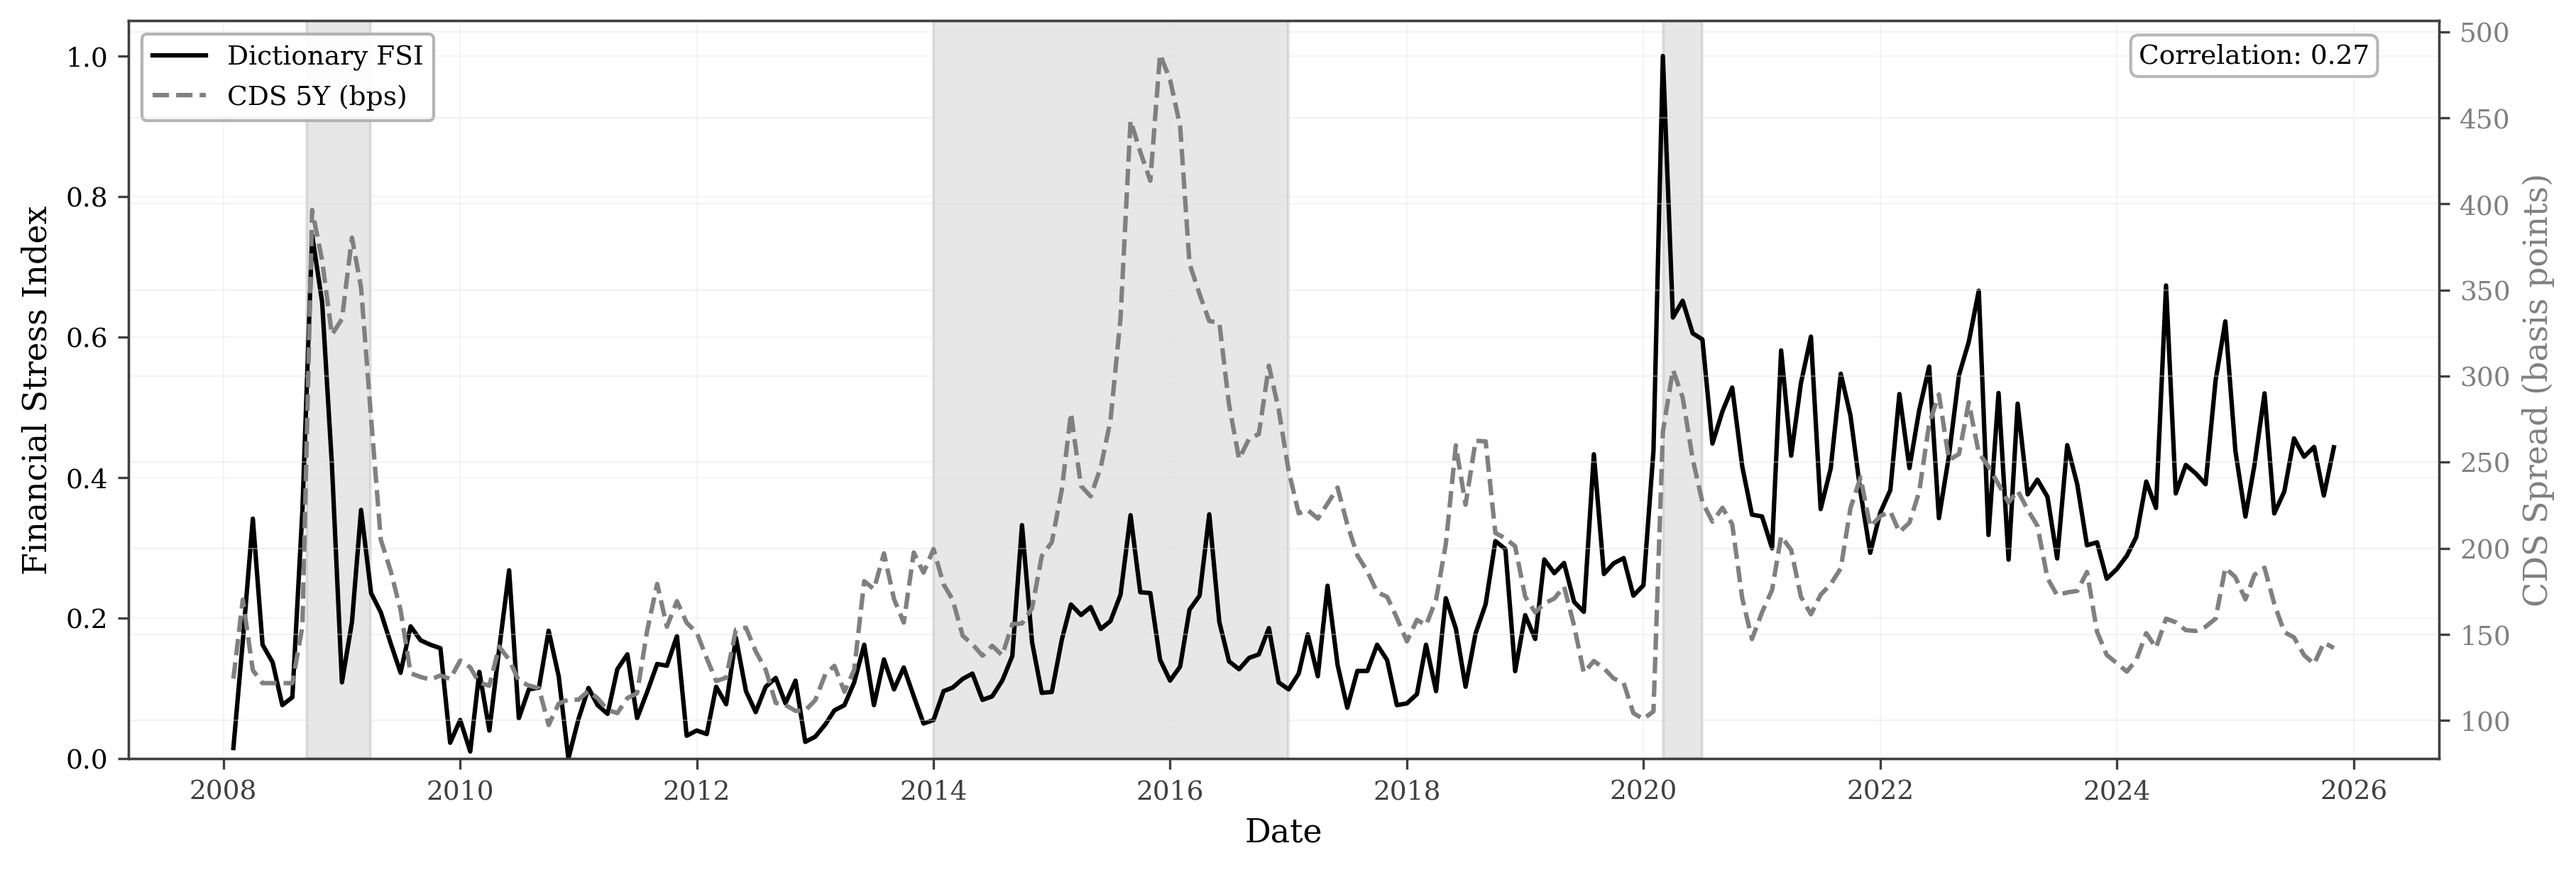
\includegraphics[width=0.95\textwidth]{../output/figures/figure_2_fsi_vs_cds_dict.png}
    \caption{Dictionary FSI and Brazil 5-Year CDS Spreads (2008--2025). Both series are shown with their respective scales (FSI on left axis, CDS on right axis). The positive co-movement supports the FSI's validity as a stress indicator.}
    \label{fig:fsi_cds}
\end{figure}

The strong performance of the Dictionary FSI relative to ML and Combined approaches carries important methodological implications. Expert-constructed query dictionaries, when carefully adapted to local language and institutional context, can outperform data-driven approaches that may overfit to idiosyncratic patterns in training data. This finding aligns with \cite{baker2016measuring}, who emphasize the value of transparent, interpretable index construction in policy-relevant applications.

\endantml:parameter>
</invoke>